\documentclass[11pt]{article}
\usepackage[margin=1in]{geometry}
\usepackage{graphicx}
\usepackage{hyperref}
\usepackage{xcolor}
\usepackage{booktabs}
\usepackage{amsmath, amssymb}
\usepackage[numbers,sort&compress]{natbib}

\hypersetup{
  colorlinks=true,
  linkcolor=blue,
  citecolor=blue,
  urlcolor=blue
}

\title{Dexter: A Memory-Centric Conversational AI Agent for Customer Support}
\author{Dashanka De Silva et al.}
\date{September 11, 2025}

\begin{document}
\maketitle

\begin{abstract}
We present Dexter, a production-ready conversational AI agent tailored for customer support. Dexter integrates a ReAct-style reasoning engine with a multi-store memory system---short-term, semantic, episodic, and procedural---to achieve continuity, personalization, and robust tool use. Unlike stateless chatbots, Dexter maintains context across sessions, extracts durable facts, and learns effective strategies from successful interactions. It exposes a FastAPI interface, supports domain tools (product search, appointment management, semantic knowledge retrieval, web search), and ships with monitoring, security, and comprehensive tests. We detail the system design, implementation, and evaluation framework, emphasizing product goals (resolution rate, CSAT proxy, latency, cost) and pragmatic engineering trade-offs. This is a living paper accompanying an evolving codebase.
\end{abstract}

\textbf{Keywords}: conversational AI, memory systems, ReAct, RAG, customer support, Pinecone, MongoDB, FastAPI, LangChain, LangGraph

\section{Introduction}
Customer support assistants must understand evolving context, remember preferences, and reliably execute tasks. Prior approaches often rely on stateless prompting or narrow flows, producing brittle behavior and impersonal experiences. Dexter addresses these limitations with: (i) a ReAct agent that plans and acts via tools; (ii) a unified memory manager spanning working, event, fact, and strategy memories; and (iii) a production surface with APIs, observability, and tests. Our goal is practical: elevate first-contact resolution and user satisfaction while controlling latency and cost.

\paragraph{Contributions} We provide: (1) a modular, memory-centric architecture that operationalizes human-like memory types in production; (2) a ReAct+LangGraph agent that integrates memory retrieval and tool execution; and (3) a product-oriented evaluation harness (tests, metrics scaffolding) for reliability and performance.

\section{Related Work}
ReAct combines step-by-step reasoning with tool calls to improve decision making and factuality\cite{yao2022react}. Retrieval-Augmented Generation (RAG) enriches responses with external knowledge retrieved by similarity search\cite{lewis2020rag}. Foundational cognitive theories describe complementary memory systems: episodic memory for events\cite{tulving1972episodic}, working memory for transient context\cite{baddeley1992working}, and procedural memory for learned skills and strategies\cite{anderson1982skill}. Recent work on memory-augmented language models further demonstrates the value of non-parametric memories to improve recall and adaptability\cite{borgeaud2022retro}.

\section{System Overview}
Dexter is a Python 3.11+ service built on FastAPI. The agent uses OpenAI models via LangChain and LangGraph. Persistence spans MongoDB (conversations, episodic/procedural) and Pinecone (semantic facts and knowledge). Short-term memory is in-process per session. Prometheus/Grafana provide observability. Docker-based workflows and AWS artifacts support deployment.

\begin{figure}[h]
  \centering
  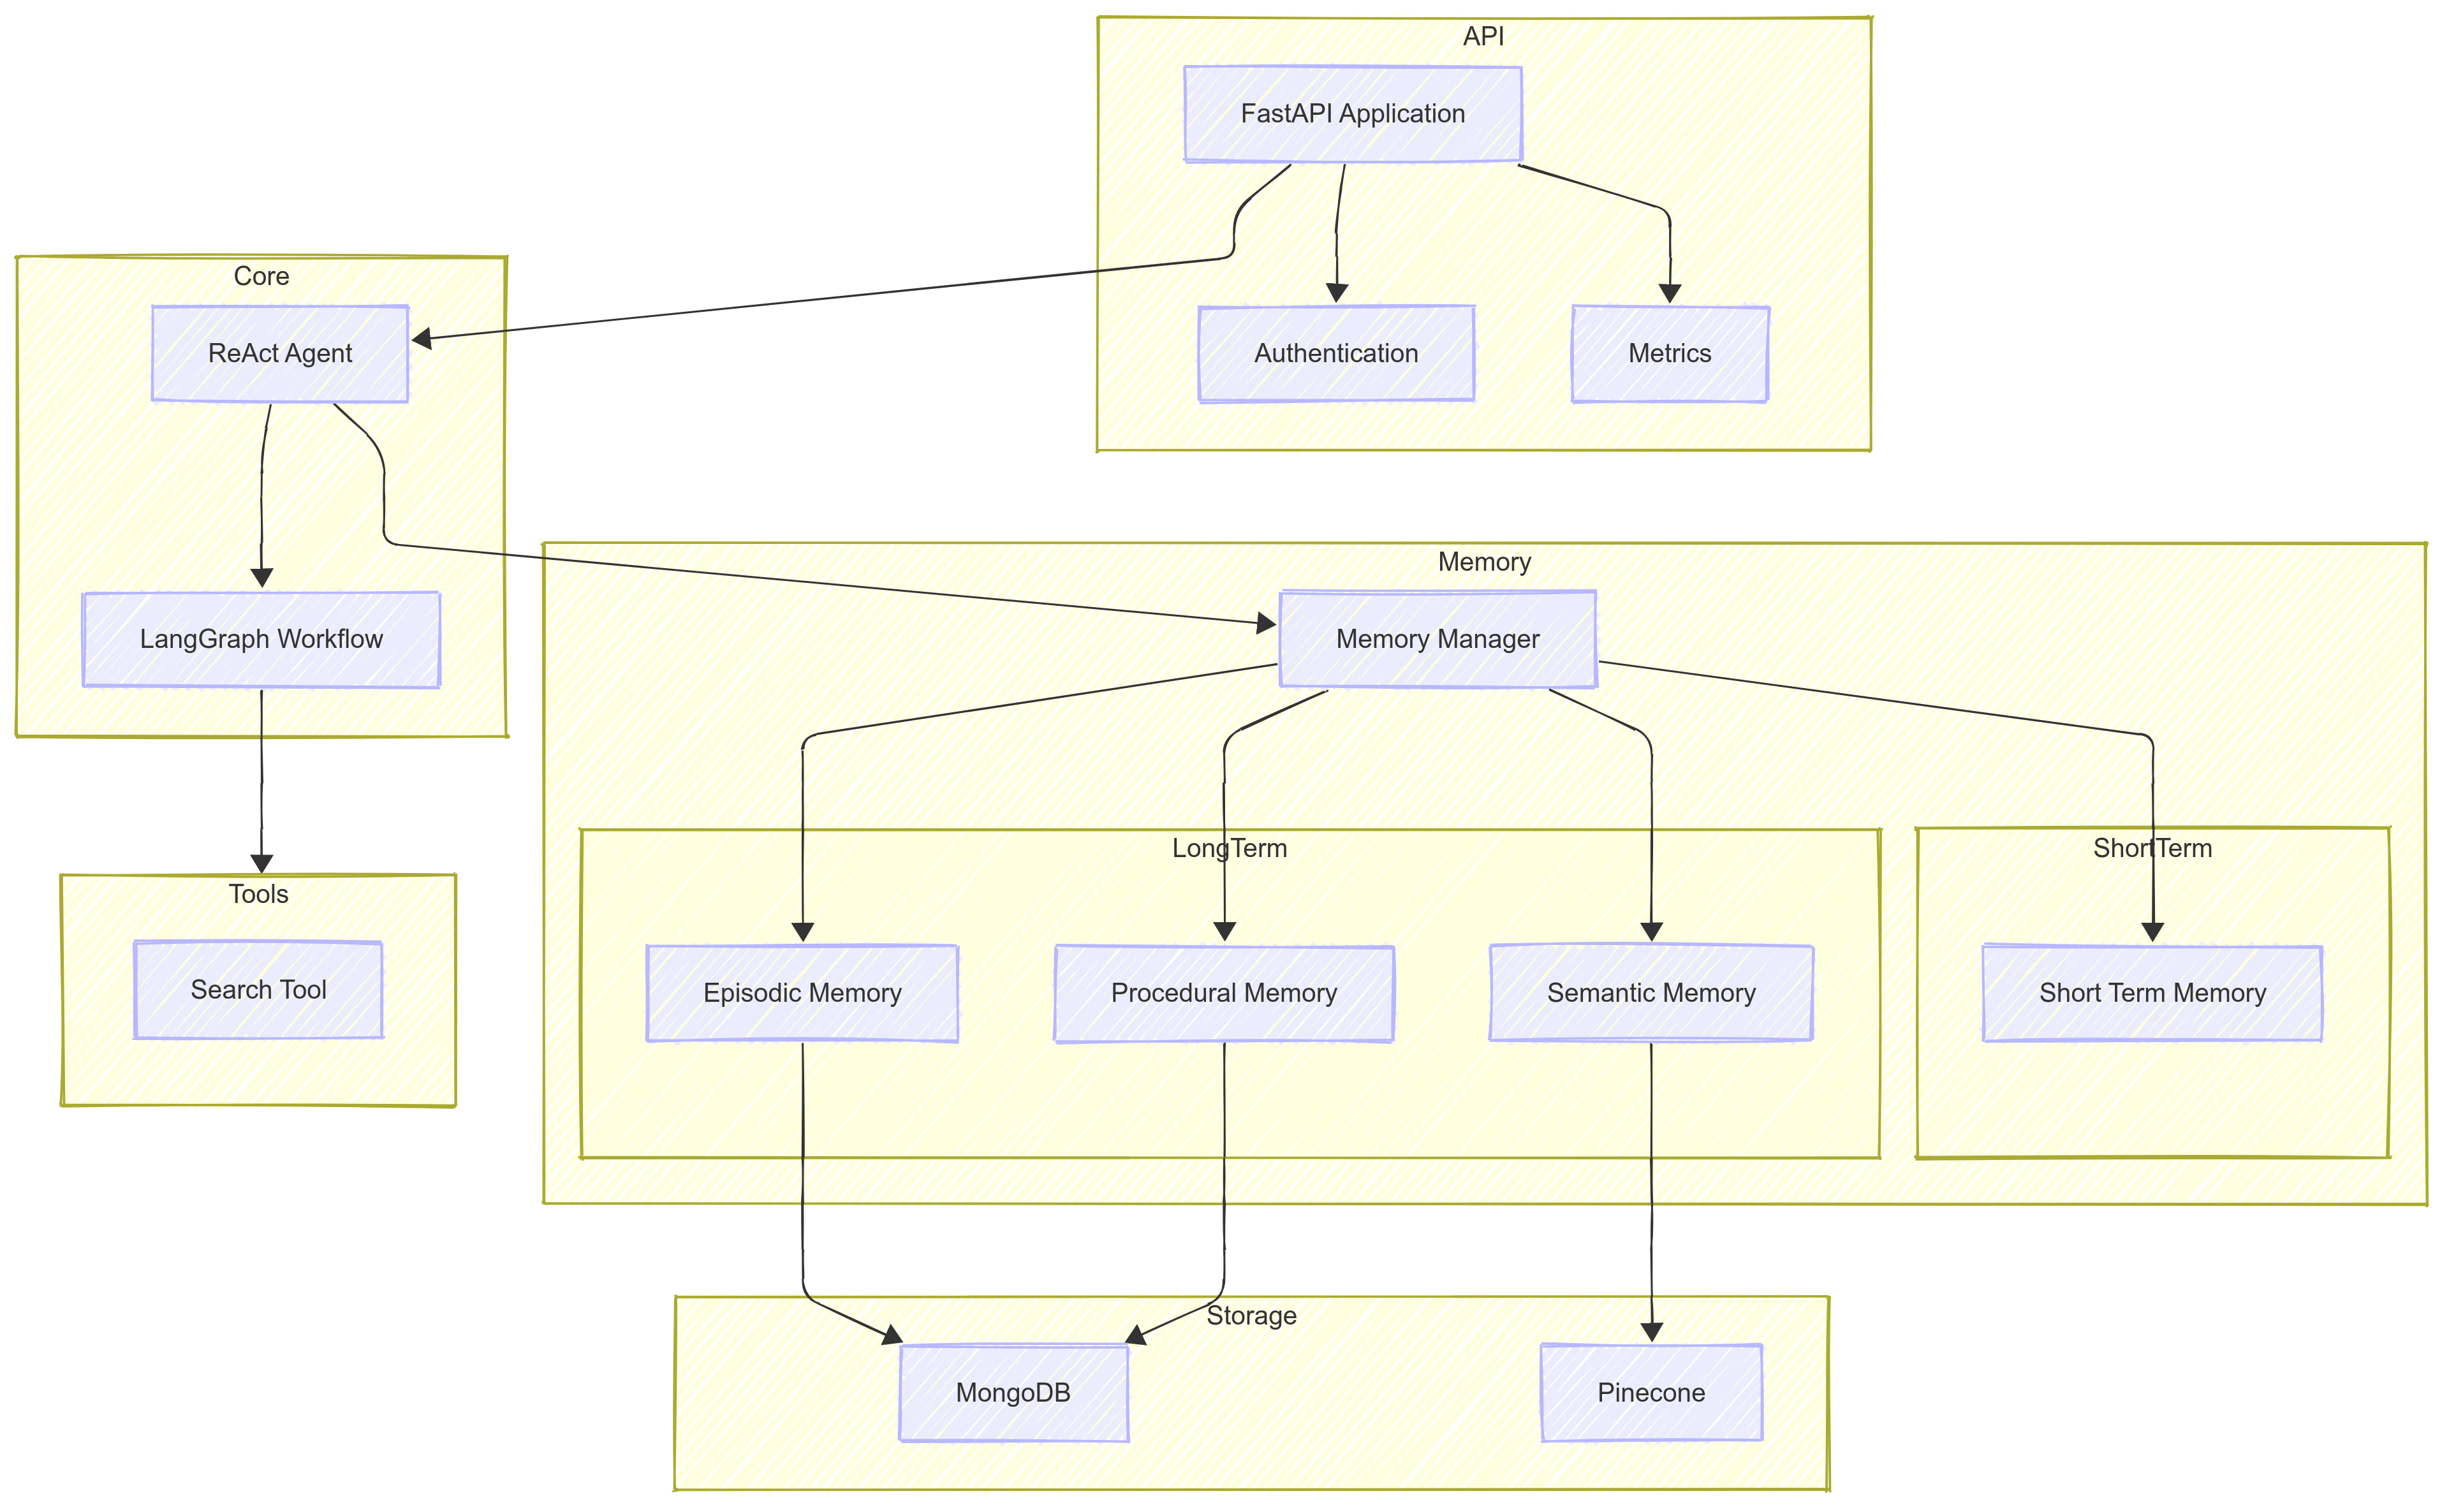
\includegraphics[width=0.95\linewidth]{../../docs/System_Architecture.png}
  \caption{System Architecture. The FastAPI agent integrates a ReAct+LangGraph controller with multi-store memory (short-term, episodic/procedural via MongoDB, semantic via Pinecone) and a tool ecosystem.}
  \label{fig:system}
\end{figure}

\section{Methods: Architecture and Algorithms}
\subsection{Memory-Oriented Architecture}
Short-term (working) memory serves as a session-scoped buffer that maintains immediate discourse context, consistent with the role of working memory in human cognition\cite{baddeley1992working}. Semantic memory captures durable, context-independent facts extracted from interaction windows and stores them as embeddings in Pinecone to enable similarity-based retrieval\cite{lewis2020rag}. Episodic memory records time-ordered conversation events and tool outcomes in MongoDB, mirroring Tulving's conception of episodic recollection\cite{tulving1972episodic}. Procedural memory retains successful strategies and tool-usage patterns---an operational analogue of skill learning\cite{anderson1982skill}---to guide future decisions.

\subsection{Agent Graph (ReAct with LangGraph)}
The agent maintains an \texttt{AgentState} (messages, identifiers, tools). The \emph{think} step composes a system prompt with tool descriptions and memory context; the model may emit \emph{tool\_calls} following the ReAct paradigm\cite{yao2022react}. A conditional edge routes to \emph{use\_tool} when tool calls exist; otherwise the response is emitted. A \emph{ToolNode} executes tools and returns their results; the loop continues until a final response is produced.

\subsection{Memory Algorithms}
For each user turn, the system assembles context by retrieving relevant semantic facts and, where appropriate, consulting episodic and procedural signals. Periodically---every $N$ messages---a semantic extractor processes a rolling window of recent messages to surface candidate facts with entities and confidence, which are then persisted with metadata for later retrieval. Following successful responses, whether tool-assisted or not, the agent materializes a procedural pattern that records the pattern type, succinct rationale, and query context, enabling future decisions to benefit from prior successes.

\section{Implementation}
\subsection{API and Contracts}
The FastAPI surface includes endpoints for chat, conversation management, memory queries (semantic/episodic/procedural), health, and metrics. Pydantic models validate inputs/outputs and timestamp messages to enforce consistent contracts.

\subsection{Tools}
The Product Search tool interprets natural-language queries using an LLM to extract structured filters (with a regex fallback), compiles MongoDB queries, and returns clearly formatted product summaries. The Appointment Management tool enforces operation-specific requirements, checks availability, performs CRUD actions, and communicates outcomes in user-friendly language. The Semantic Retrieval tool queries Pinecone to surface relevant knowledge, returning grounded content with source attribution and similarity scores. A Web Search tool complements internal knowledge by providing an external retrieval path for open-domain information when appropriate.

\subsection{Storage and Configuration}
MongoDB stores conversations, episodic events, and procedural patterns with metadata. Pinecone stores semantic facts and knowledge documents with per-user scoping and metadata to enable filtered retrieval. Configuration is environment-driven (OpenAI, Pinecone, MongoDB, metrics, prompt path).

\section{Evaluation (Product-Oriented)}
Objectives include resolution rate (fraction of sessions resolved), a CSAT proxy (readability and task completion signals), p95 latency under nominal load, and cost (token and tool usage). Methodology combines unit/integration tests, performance testing, and observability via Prometheus counters and histograms; coverage tooling and dashboards support CI gating.

\section{Case Studies}
Use cases include product discovery (price- and feature-aware search that recalls preferences), appointment workflows (end-to-end booking and rescheduling guided by learned patterns), and knowledge questions (RAG-like responses grounded in internal knowledge, with web search fallback).

\section{Limitations and Future Work}
Session-level knowledge consolidation and spaced rehearsal are deferred. Failure-aware procedural learning can be expanded to adaptive retries and guarded parameter suggestions. Access control and multi-tenancy can be strengthened via middleware and database scoping patterns; privacy filters for retrieval are planned.

\section{Conclusion}
Dexter operationalizes multi-memory conversational AI in a production setting. By unifying ReAct planning, tool use, and memory orchestration under a clean API and observability stack, it provides a practical foundation for customer support automation with measurable outcomes.

\paragraph{Acknowledgments} Built with FastAPI, LangChain/LangGraph, OpenAI, MongoDB, and Pinecone. We thank the open-source community and contributors.

\bibliographystyle{plainnat}
\bibliography{refs}

\end{document}


